\subsection{The opportunity and cost of local reuse}
\label{sec:motivation}
The preceding approaches show that efficient local arithmetic and intelligent
scheduling are both available. The remaining difficulty is choosing their
boundary. How much dependent work should one local unit absorb, and how much
independent work should remain available to other units?
An \textbf{execution organization} determines which operations run together,
where values live, how producers present them to successors, and when dependent
work can begin. An arithmetic core implements a local function. Its
organization determines the communication and resources needed to compose
that function into a complete transform.

\begin{figure*}[t]
\centering
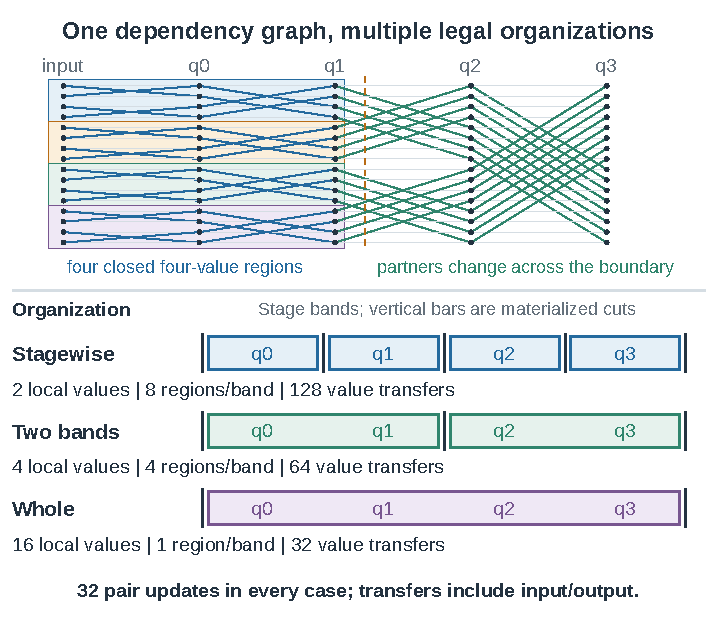
\includegraphics[width=\textwidth]{figures/drawio/exports/organization_tradeoffs.pdf}
\caption{Three organizations of the same 16-point Hadamard graph. Boxes enclose
closed components, not fixed CUDA blocks. Rows are reordered within each band
to display closure, so equal row positions across a cut need not be the same
logical value. All alternatives execute 32 pairs. Value-only reads and writes
total 128, 64, and 32 transfers per transform. Deeper bands enlarge components
and reduce their count. These analytical counts imply neither measured
speedup nor a hardware occupancy guarantee.}
\label{fig:organization-tradeoffs}
\end{figure*}

Figure~\ref{fig:organization-tradeoffs} makes the choice concrete using the
same 16-point Hadamard graph. A stage-at-a-time organization exposes eight
independent pairs but reads and writes all values at each stage. Grouping
two stages retains four values per local subgraph and halves materialized
value traffic. Retaining all four stages minimizes this traffic but leaves
only one independent whole-transform component per batch instance.
The arithmetic work is unchanged. These counts expose a trade-off rather
than a winner, because a component may itself use multiple cooperating threads
and its resource cost depends on the selected core.

The roofline opportunity follows from this distinction. For $B$ transforms of
length $N=2^L$, let $e$ be bytes per value and $G$ the number of materialized
stage groups. There are $BNL/2$ pair updates. If each group reads and writes
the array once, ideal value-only intensity is
\begin{equation}
I_{\mathrm{value}}\simeq\frac{L}{4eG}.
\label{eq:intensity}
\end{equation}
At a selected storage boundary, actual intensity is pair work divided by
transferred bytes. Its roofline ceiling is the smaller of core throughput and
bandwidth times intensity. Coefficients, transactions, cache reuse, and spills
change the traffic, while synchronization and execution efficiency determine
the distance below this ceiling.

\begin{figure}[t]
\centering
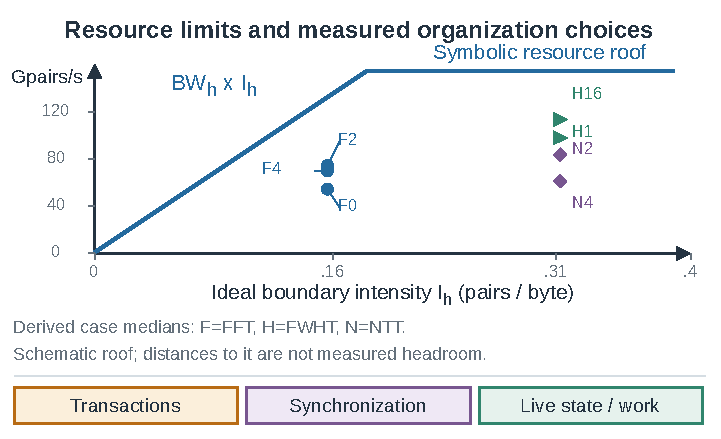
\includegraphics[width=\columnwidth]{figures/drawio/exports/roofline.pdf}
\caption{Schematic boundary roofline. Boundary intensity determines the
bandwidth ceiling, while the arithmetic core determines the compute ceiling.
Attaining either also requires sufficient ready subgraphs, resident resources,
and valid synchronization. Axes are symbolic. The lower panel states
attainment conditions, not a measured occupancy model.}
\label{fig:roofline}
\end{figure}

Reducing $G$ raises ideal intensity but enlarges live state, potentially reducing
occupancy and independent work. A faster core raises the compute ceiling
without removing a bandwidth limit. Conversely, enough arithmetic work per
byte does not ensure enough ready work to fill the machine. The ordinary
roofline identifies a resource ceiling, not a schedule that reaches it.
\textbf{The mapping must jointly choose
local reuse and enough parallel work to sustain it.}

A controlled historical V100 NTT pair illustrates the workload dependence.
At $N=2^{20}$ and batch 16, assigning two four-warp row subgraphs per CTA
instead of one improved throughput by approximately $1.154\times$ with the
same register continuation. At batch four, the change slowed execution.
The result motivates workload-dependent organization rather than a universal
preference for more local work. In particular, batch and local component size
cannot be tuned independently even when the arithmetic core is unchanged.

\subsection{Why a hierarchy and a common construction}
This trade-off suggests retaining a bounded amount of dependent computation
while exposing the remaining independent work. Stage and data positions
provide two allocation axes. A worker may execute
several stages over time, or distinct resources may serve successive stages.
Independent components may occupy different workers or reuse a worker
sequentially. Combining these choices retains a bounded region while streaming
independent work through it. We call their combination \textbf{hybrid dataflow}.
A stagewise schedule and a spatial stage pipeline are useful endpoints of
these choices, not the only organizations the framework should express.

The choice recurs across registers, cooperating threads, and groups staged
through global memory. \textbf{Hierarchy removes a fixed-capacity expression
limit.}
When a transform exceeds what a fixed number of bounded bands can express,
additional bands or recursive refinement retain the same construction.
Logical depth, materialized group count, and hardware storage levels are
therefore distinct. More levels express larger workloads but create no
additional bandwidth or storage.

More batch provides independent work to amortize startup and cover transfers.
Realizing that slack still requires lookahead, finite buffers, and available
resources. A successor needs its actual predecessor set, not merely a
contiguous prefix of producer output. The method must therefore derive both
locality and readiness from the graph.

Stage-bit dependencies provide that stable description. Changing arithmetic
alters operation labels, changing length reinstantiates the dependency domain,
and changing GPU alters feasible resources and service rates. This motivates
separate \textbf{semantics, workload, and hardware} inputs without separating
their performance effects. The separation answers a practical scaling problem.
Increasing $N$ or batch should instantiate a new work domain rather than
require a new operator implementation. Changing arithmetic should replace
compatible local functions rather than rederive the surrounding dependencies.
Changing GPU should alter feasible mappings and service costs rather than
the mathematical request.

These observations give the method three obligations. It must derive a legal
local unit, connect such units without losing dependencies or value identity,
and repeat the organization when a workload exceeds one storage scope.
The next section develops those rules. Block-level and resident subgraph
execution then provide their concrete GPU realization.
